%--------------------------------------------------------------------%
%
% Berkas utama templat LaTeX.
%
% author Petra Barus, Peb Ruswono Aryan
% updated by Dionesius Agung (2020)
% adapted by Irfan Tito Kurniawan (2020)
% adapted for ET by Rama Rahardi (2021)
%--------------------------------------------------------------------%
%
% Berkas ini berisi struktur utama dokumen LaTeX yang akan dibuat.
%
%--------------------------------------------------------------------%
\documentclass[12pt, a4paper, onecolumn, oneside, final]{report}

%-------------------------------------------------------------------%
%
% Konfigurasi dokumen LaTeX untuk laporan tesis IF ITB
%
% @author Petra Novandi
% updated by Dionesius Agung (2020)
% adapted by Irfan Tito Kurniawan (2020)
% adapted for ET by Rama Rahardi (2021)
%-------------------------------------------------------------------%
%
% Berkas asli berasal dari Steven Lolong
%
%-------------------------------------------------------------------%

%%%%%%%%%%%%%%%%%%%%%%%%%%%%%%%%%%%%
%  DOCUMENT LAYOUT AND FORMATTING  %
%%%%%%%%%%%%%%%%%%%%%%%%%%%%%%%%%%%%
% Document layout
\usepackage[top=3cm,bottom=3cm,left=4cm,right=3cm,a4paper]{geometry}

% Uncomment these two packages if you want to use
%  the Times New Roman font for your document
\usepackage{mathptmx}
\usepackage{newtxtext}

% Judul bahasa Indonesia
\usepackage[bahasa]{babel}
% \usepackage[english]{babel}

% Spacing 1.5
\usepackage{setspace}
\renewcommand{\baselinestretch}{1.5}

% Prevent overfull (or underfull) if possible
%\setlength{\emergencystretch}{25pt}

% Avoid widow and orphan lines if possible
\widowpenalty500
\clubpenalty10000

% Hyphenation penalty
%--------------------------------------------------------------------%
%
% Hyphenation untuk Bahasa Indonesia
%
% @author Petra Barus
%
%--------------------------------------------------------------------%
%
% Secara otomatis LaTeX dapat langsung memenggal kata dalam dokumen,
% tapi sering kali terdapat kesalahan dalam pemenggalan kata. Untuk
% memperbaiki kesalahan pemenggalan kata tertentu, cara pemenggalan
% kata tersebut dapat ditambahkan pada dokumen ini. Pemenggalan
% dilakukan dengan menambahkan karakter '-' pada suku kata yang
% perlu dipisahkan.
%
% Contoh pemenggalan kata 'analisa' dilakukan dengan 'a-na-li-sa'
%
%--------------------------------------------------------------------%

\hyphenation {
	% A
	%
	a-na-li-sa
	a-pli-ka-si

	% B
	%
	be-be-ra-pa
	ber-ge-rak

	% C
	%
	ca-ri

	% D
	%
	da-e-rah
	di-nya-ta-kan
	de-fi-ni-si

	% E
	%
	e-ner-gi
	eks-klu-sif

	% F
	%
	fa-si-li-tas

	% G
	%
	ga-bung-an

	% H
	%
	ha-lang-an

	% I
	% 
	i-nduk

	% J
	%
	ka-me-ra
	kua-li-tas

	% K
	%

	% L
	%

	% M
	%

	% N
	%

	% O
	%

	% P
	%

	% Q
	%

	% R
	%

	% S
	%

	% T
	% 

	% U
	%

	% V
	%

	% W
	%

	% X
	%

	% Y
	% 

	% Z
	%
}

\hyphenpenalty=10000
\tolerance=1
\sloppy

%%%%%%%%%%%%%%%%%%%%%%%%%%%%%%%
%  BIBLIOGRAPHY AND CITATION  %
%%%%%%%%%%%%%%%%%%%%%%%%%%%%%%%

%%%%%%%%%%%%%%
%  PACKAGES  %
%%%%%%%%%%%%%%
\usepackage[utf8]{inputenc}
\usepackage{graphicx}
\usepackage{titling}
\usepackage{outlines}
\usepackage{blindtext}
\usepackage{sectsty}
\usepackage{chngcntr}
\usepackage{etoolbox}
\usepackage{hyperref}
\usepackage{titlesec}
\usepackage{parskip}
\usepackage{booktabs}
\usepackage{tabularx}
\usepackage[chapter]{algorithm}
\usepackage{algpseudocode}
\usepackage{comment}
\usepackage{cite}
\usepackage{amssymb}
\usepackage{pifont}
% \usepackage{mathabx}
\usepackage{array, makecell}
% \usepackage{apacite}
\usepackage{natbib}
% \usepackage{svg}
\usepackage[inkscapearea=page]{svg}
\renewcommand\theadfont{\bfseries}
% \usepackage{apalike}

%%%%%%%%%%%%%%$$%%%%%%%%%
%  CHAPTER AND SECTION  %
%%%%%%%%%%%%%%%%$$%%%%%%%
% Format judul bab
\chapterfont{\centering \large}
\titleformat{\chapter}[hang] %[display]
{\large\centering\bfseries}
{\chaptertitlename\ \Roman{chapter} }{0em}
{\large\bfseries\MakeUppercase}
\titlespacing*{\chapter}
{0pt}
{-1.5\baselineskip}
{1\baselineskip}

% Format judul section (dan sub(sub)section)
\titleformat*{\section}{\bfseries\normalsize}
\titleformat*{\subsection}{\bfseries\normalsize}
\titleformat*{\subsubsection}{\bfseries\normalsize}
\titlespacing*{\section}{0pt}{2ex}{0pt}
\titlespacing*{\subsection}{0pt}{2ex}{0pt}
\titlespacing*{\subsubsection}{0pt}{2ex}{0pt}

% Kedalaman hierarki section (paling dalam subsubsection)
\setcounter{secnumdepth}{3}


%%%%%%%%%%%%%%%%%%%%%%%%%%%%%%%%%%%%%%%%%%%%%%%%%%
%  TABLE OF CONTENTS, LISTS OF FIGURES & TABLES  %
%%%%%%%%%%%%%%%%%%%%%%%%%%%%%%%%%%%%%%%%%%%%%%%%%%
\usepackage[titles]{tocloft}
\usepackage[titletoc]{appendix}
\usepackage{tocbibind}

% Kedalaman hierarki maksimum ToC
% (yang masuk ToC hanya sampai subsection: I.1.1.)
\setcounter{tocdepth}{2}

% Hilangkan gap antar-bab di ToC
\setlength{\cftbeforechapskip}{0pt}

% Tambah kata "BAB" sebelum nomor bab di daftar isi
% TODO: still problematic when used with list of appendices (uncomment these 4 following lines to reproduce the problem)
% \renewcommand{\cftchappresnum}{BAB~} % BAB before number in ToC
% \newlength{\mylen} % a scratch length
% \settowidth{\mylen}{\bfseries\cftchappresnum\cftchapaftersnum} % extra space
% \addtolength{\cftchapnumwidth}{\mylen} % add the extra space

% Pisah daftar lampiran dari ToC
%%%
\renewcommand{\appendixtocname}{Daftar Lampiran}

\makeatletter
\let\oldappendix\appendices

\renewcommand{\appendices}{%
	\clearpage
	% From now, everything goes to the app file and not to the toc
	\let\tf@toc\tf@app
	\addtocontents{app}{\protect\setcounter{tocdepth}{1}}
	\immediate\write\@auxout{%
		\string\let\string\tf@toc\string\tf@app^^J
	}
	\oldappendix
}%

\newcommand{\listofappendices}{%
	\begingroup
	\renewcommand{\contentsname}{\appendixtocname}
	\let\@oldstarttoc\@starttoc
	\def\@starttoc##1{\@oldstarttoc{app}}
	% Reusing the code for \tableofcontents with different
	%   \contentsname and different file handle app
	\tableofcontents
	\endgroup
}
\makeatother
%%%

% Hilangkan gap antara entri gambar & tabel antarbab di daftar tabel 
% dan daftar gambar (hanya terlihat kalau ada gambar/tabel di >1 bab)
\newcommand*{\noaddvspace}{\renewcommand*{\addvspace}[1]{}}
\addtocontents{lof}{\protect\noaddvspace}
\addtocontents{lot}{\protect\noaddvspace}

%%%%%%%%%%%%%%%%%%%%%%%%%%%%%%%%%%%%%%%%%
%  FLOATS: FIGURES, TABLES, ALGORITHMS  %
%%%%%%%%%%%%%%%%%%%%%%%%%%%%%%%%%%%%%%%%%
% Before:
% ---
% Counter untuk figure dan table.
% \counterwithin{figure}{section}
% \counterwithin{table}{section}
% ---

\usepackage[labelsep=period,
justification=justified,
format=hang]{caption}
\usepackage[labelformat=simple]{subcaption}
%% Hack subfigure cross-ref agar pakai tanda kurung
%%   e.g. Gambar II.2(a), bukan Gambar II.2a
%% (method recommended in subcaption package documentation)
\renewcommand\thesubfigure{(\alph{subfigure})}

% Counter untuk gambar dan tabel
\renewcommand*{\thefigure}{\Roman{chapter}-\arabic{figure}}
\renewcommand*{\thetable}{\Roman{chapter}-\arabic{table}}

% Jarak spasi antara float dengan teks utama
\captionsetup[figure]{belowskip=-1em}
\captionsetup[subfigure]{belowskip=0pt}
\setlength{\textfloatsep}{2\baselineskip}
\setlength{\intextsep}{2\baselineskip}

% Spasi single di environment table
\AtBeginEnvironment{table}
{\renewcommand{\baselinestretch}{1.0}}

% Font lebih kecil untuk tabel
\AtBeginEnvironment{tabular}
{\small}

% Spasi single di environment algorithm
\AtBeginEnvironment{algorithm}
{\renewcommand{\baselinestretch}{1.0}}

% Rename "Algorithm" into "Algoritma"
\makeatletter
\renewcommand*{\ALG@name}{Algoritma}
\newcommand{\algorithmname}{\ALG@name}
\makeatother


%%%%%%%%%%%%%%%%%%%%%%%%%
%  MATHS AND EQUATIONS  %
%%%%%%%%%%%%%%%%%%%%%%%%%
\usepackage{amsmath}
\usepackage{amsfonts}
\usepackage{mathtools}

% Counter untuk equation
\renewcommand*{\theequation}{\Roman{chapter}.\arabic{equation}}

% Allow page breaks on long equations
\allowdisplaybreaks[1-4]

% Operator dan notasi custom tambahan
% contoh: argmin dan argmax
\DeclareMathOperator*{\argmax}{argmax}
\DeclareMathOperator*{\argmin}{argmin}
% contoh: notasi bayes p(x | y)
\newcommand{\bayes}[2]{p(#1 \mid #2)\xspace}

%%%%%%%%%%%%%%%%%
%  GANTT CHART  %
%%%%%%%%%%%%%%%%%
\usepackage{changepage}
\usepackage{pgfgantt}
\ganttset{calendar week text={\currentweek}}

%%%%%%%%%%%%%%
%  DIAGRAMS  %
%%%%%%%%%%%%%%
\usepackage{tikz}
\usetikzlibrary{shapes, arrows, fit}
\tikzstyle{block} = [rectangle, draw, minimum height=3em, minimum width=6em, text centered]
\tikzstyle{pinstyle} = [pin edge={to-, thin, black}]
\tikzstyle{input} = [coordinate]
\tikzstyle{output} = [coordinate]

%%%%%%%%%%%%%%%%%%%%%%%%%%%%%%%%
%  GLOSSARY AND ABBREVIATIONS  %
%%%%%%%%%%%%%%%%%%%%%%%%%%%%%%%%
% Load package acronym dan indexonlyfirst untuk hanya 
% menunjukkan kemunculan pertama singkatan
\usepackage[nomain, abbreviations, indexonlyfirst]{glossaries-extra}

% Buat glossary baru khusus untuk lambang
\newglossary[slg]{symbols}{syi}{syg}{Daftar Lambang}

% Buat glossary
\makeglossaries

% Hilangkan judul dari glossary
\renewcommand{\glossarysection}[2][]{}

% Style glossary untuk Daftar Singkatan
\newglossarystyle{daftarsingkatan}{
	% Dasarkan style pada style long3colheader
	\setglossarystyle{long3colheader}
	
	\renewenvironment{theglossary}{\begin{longtable}{p{2cm}p{\glsdescwidth}p{\glspagelistwidth}}}{\end{longtable}}
	
	% Ganti header glossary
	\renewcommand{\glossaryheader}{
		\centering \textbf{SINGKATAN} &
		\centering \textbf{NAMA} &
		\centering \textbf{KEMUNCULAN PERTAMA}
		\endhead
	}
	
	% Ganti lebar kolom glossary
	\renewcommand{\glsdescwidth}{7cm}
	\renewcommand{\glspagelistwidth}{4cm}
	
	% Buat line break dalam sel menjadi 1 spasi
	\renewcommand{\baselinestretch}{1.0} 
	\renewcommand{\arraystretch}{1.5}
	\selectfont
	
	% Ganti isi glossary menjadi singkatan - deskripsi - kemunculan pertama
	\renewcommand{\glossentry}[2]{
		\glsentryitem{##1}\glstarget{##1}{\glossentryname{##1}} 
		& \glossentrydesc{##1}
		& \centering ##2
		\tabularnewline
	}
	
	\renewcommand{\glsgroupskip}{}
}

% Style glossary untuk Daftar Lambang
\newglossarystyle{daftarlambang}{
	% Dasarkan style pada style long3colheader
	\setglossarystyle{long3colheader}
	% Hack untuk mengubah lebar kolom lambang
	\renewenvironment{theglossary}{\begin{longtable}{p{2cm}p{\glsdescwidth}p{\glspagelistwidth}}}{\end{longtable}}
	% Ganti header glossary
	\renewcommand{\glossaryheader}{
		\centering \textbf{LAMBANG} &
		\centering \textbf{NAMA} &
		\centering \textbf{KEMUNCULAN PERTAMA}
		\endhead
	}
	
	% Ganti lebar kolom glossary
	\renewcommand{\glsdescwidth}{7cm}
	\renewcommand{\glspagelistwidth}{4cm}
	
	% Buat line break dalam sel menjadi 1 spasi
	\renewcommand{\baselinestretch}{1.0} 
	\renewcommand{\arraystretch}{1.5}
	\selectfont
	
	% Ganti isi glossary menjadi lambang - deskripsi - kemunculan pertama
	\renewcommand{\glossentry}[2]{
		\glsentryitem{##1}\glstarget{##1}{\glossentryname{##1}} 
		& \glossentrydesc{##1}
		& \centering ##2
		\tabularnewline
	}
	
	\renewcommand{\glsgroupskip}{}
}

\makeatletter

\makeatother

\begin{document}

    %Basic configuration
    % \title{Enhancing Video Analytics Accuracy via
    % Real-time Automated Video Compression Parameter Tuning as
    % well as Enabling Resource Allocator}
    % \title{Pengembangan Desain Sistem \emph{Resource Allocator} 
    % Berbasis Sensitivitas untuk Meningkatkan Akurasi pada Aplikasi
    % \emph{Video Analytics}}
    \title{Pengembangan Desain Sistem \emph{Sensitivity-based Resource Allocator} 
    untuk Meningkatkan Akurasi pada Aplikasi
    \emph{Video Analytics}}
    % Pengembangan desain sistem Resource Allocator berbasis sensitivitas untuk meningkatkan akurasi pada
    % Aplikasi Video Analytics
    \date{\today}
    \author{
        Faishal Zharfan \\
        NIM: 18119002
    }

    \pagenumbering{roman}
    \setcounter{page}{0}

    \clearpage
\pagestyle{empty}

% Setting margin for cover page
\newgeometry{top=3cm,bottom=3cm,left=3cm,right=3cm}

% Use Times font for cover page as per the thesis document guidelines
%{\fontfamily{ptm}\selectfont%
\begin{center}
    
    \smallskip
	\renewcommand{\baselinestretch}{1}
	
    \large{\bfseries \MakeUppercase{\thetitle}}
    \\[5\baselineskip]

    \large{\bfseries TUGAS AKHIR}
    \\[\baselineskip]
	
    \normalsize{ \bfseries
    	Karya tulis sebagai salah satu syarat\\
    	untuk memperoleh gelar Sarjana dari\\
    	Institut Teknologi Bandung
	}
    \\[3\baselineskip]

    \normalsize{ \bfseries Oleh\\}
    \large{ 
    	\bfseries \MakeUppercase{\theauthor}\\
    	(Program Studi Teknik Telekomunikasi)
	}

    \vfill
    \begin{figure}[h]
        \centering
      	
\includegraphics[height=3.5cm,keepaspectratio]{resources/cover-ganesha.jpg}
    \end{figure}
    \vfill

    \large{ \bfseries
	    \uppercase{
	        Institut Teknologi Bandung\\
	    }
    	Mei 2024
	}

\end{center}
%}%

\restoregeometry
\clearpage

    \clearpage
\chapter*{Abstrak}
\addcontentsline{toc}{chapter}{ABSTRAK}

\begin{center}
	\linespread{1}
	\large{\bfseries{
			\MakeUppercase\thetitle
		}
	}\\[1\baselineskip]
	
	\normalsize{Oleh\\}
	\large{ 
		\bfseries \theauthor\\
		(Program Studi Teknik Telekomunikasi)
	}\\[2\baselineskip]
\end{center}

\medskip

\begin{spacing}{1.0}
	
	%taruh abstrak bahasa indonesia di sini
	\blindtext
	
	\blindtext
	
	\textit{Kata kunci: pertama, kedua, ketiga.}
	
\end{spacing}

\clearpage

	\clearpage
\chapter*{Abstract}
\addcontentsline{toc}{chapter}{\textit{ABSTRACT}}

\begin{center}
	\linespread{1}
	\large{\bfseries{
			\MakeUppercase{\textit{The Development of Sensitivity-based Resource Allocator 
			System to Enhance Video Analytics Applications Accuracy}}
		}
	}\\[1\baselineskip]
	% Pengembangan Desain Sistem Sensitivity-based Resource Allocator 
	% 		untuk Meningkatkan Akurasi pada Aplikasi
	% 		Video Analytics
	\normalsize{\textit{By}\\}
	\large{ 
		\bfseries \theauthor\\
		(\textit{\underline{Telecommunication Engineering Program}})
	}\\[2\baselineskip]
\end{center}

\medskip

\begin{spacing}{1.0}
	
	%taruh abstrak bahasa inggris di sini bila diperlukan
	\LaTeX lorem ipsum \citep{dds}, \citep{videostorm}, \citep{concierge}
	\itshape{
		\blindtext
		
		\blindtext
		
		Keywords: first, second, third.
	}
\end{spacing}

\clearpage

    \clearpage
\pagestyle{empty}

\begin{center}
	\renewcommand{\baselinestretch}{1}
    \large{\bfseries \MakeUppercase{\thetitle}}
    \\[2\baselineskip]
	
    \normalsize{Oleh\\
    \textbf{\theauthor}\\
    \textbf{(Program Studi Sarjana Teknik Telekomunikasi)}
    \\[\baselineskip]
    Institut Teknologi Bandung}
    \\[3\baselineskip]

    \normalsize{Menyetujui\\
    Tim Pembimbing
    \\[\baselineskip]
    
    Tanggal \thedate\\[2\baselineskip]
    Ketua\\[4\baselineskip]
    \rule{5cm}{0.4pt} \\
    Prof. Ir. Hendrawan, M.Sc., Ph.D.\\
    NIP. 196007051987021002}

\end{center}
\clearpage

    \clearpage
%\pagestyle{empty}

\begin{center}    
	\renewcommand{\baselinestretch}{1}
    \large{\bfseries \MakeUppercase{\thetitle}}
    \\[2\baselineskip]

\large{\bfseries HALAMAN PENGESAHAN}
    \\[\baselineskip]

    \normalsize{Oleh\\
    	\textbf{\theauthor}\\
    	\textbf{(Program Studi Teknik Telekomunikasi)}
    	\\[\baselineskip]
    	Institut Teknologi Bandung}
    \\[3\baselineskip]
    
    
    % \normalsize{Menyetujui\\
    % 	Tim Pembimbing
    % 	\\[\baselineskip]
    % 	Tanggal \thedate}
    % \\[5\baselineskip]
    
    % \normalsize{%
    % \setlength{\tabcolsep}{12pt}
    % \begin{tabular}{}
    %     Ketua \\
    %     \rule{5cm}{0.4pt} \\
    %     Nama dan Gelar Pembimbing I \\
    %     NIP. 123456789  \\
    % \end{tabular}
    % }
    
    \normalsize{Menyetujui\\
    Tim Pembimbing
    \\[\baselineskip]
    
    Tanggal \thedate\\[2\baselineskip]
    Ketua\\[4\baselineskip]
    \rule{5cm}{0.4pt} \\
    Prof. Ir. Hendrawan, M.Sc., Ph.D.\\
    NIP. 196007051987021002}

\end{center}
\clearpage

    \clearpage
\chapter*{Pedoman Penggunaan Tugas Akhir}
\addcontentsline{toc}{chapter}{PEDOMAN PENGGUNAAN TUGAS AKHIR}

Tugas Akhir Sarjana yang tidak dipublikasikan terdaftar dan tersedia di Perpustakaan Institut Teknologi Bandung, dan terbuka untuk umum dengan ketentuan bahwa hak cipta ada pada penulis dengan mengikuti aturan HaKI yang berlaku di Institut Teknologi Bandung. Referensi kepustakaan diperkenankan dicatat, tetapi pengutipan atau peringkasan hanya dapat dilakukan seizin penulis dan harus disertai dengan kaidah ilmiah untuk menyebutkan sumbernya.

Sitasi hasil penelitian Tugas Akhir ini dapat ditulis dalam bahasa Indonesia sebagai berikut:

\hangindent=1.27cm Zharfan, Faishal. (\the\year): \textit{\thetitle}, Tugas Akhir Program Sarjana, Institut Teknologi Bandung\\

dan dalam bahasa Inggris sebagai berikut:

\hangindent=1.27cm Zharfan, Faishal. (\the\year): \textit{The Development of Sensitivity-based Resource Allocator 
System to Enhance Video Analytics Applications Accuracy}, Undergraduate Final Year Project, Institut Teknologi Bandung\\

Memperbanyak atau menerbitkan sebagian atau seluruh Tugas Akhir haruslah seizin Dekan Sekolah Teknik Elektro dan Informatika Institut Teknologi Bandung.

\clearpage
    \clearpage

\begin{center}
    \topskip0pt
    \vspace*{\fill}
    \textit{
    Jangan bingung\\
    Tidak usah repot-repot
    }
    \vspace*{\fill}
\end{center}

\clearpage

    \pagestyle{plain}

    % Frontmatter
    \chapter*{Kata Pengantar}
\addcontentsline{toc}{chapter}{KATA PENGANTAR}

%Gunakan bagian ini untuk memberikan ucapan terima kasih kepada semua pihak yang secara langsung atau tidak langsung membantu penyelesaian tugas akhir, termasuk pemberi beasiswa jika ada. Utamakan untuk memberikan ucapan terima kasih kepada tim pembimbing tugas akhir dan staf pengajar atau pihak program studi, bahkan sebelum mengucapkan terima kasih kepada keluarga. Ucapan terima kasih sebaiknya bukan hanya menyebutkan nama orang saja, tetapi juga memberikan penjelasan bagaimana bentuk bantuan/dukungan yang diberikan. Gunakan bahasa yang baik dan sopan serta memberikan kesan yang enak untuk dibaca. Sebagai contoh: “Tidak lupa saya ucapkan terima kasih kepada teman dekat saya, Tito, yang sejak satu tahun terakhir ini selalu memberikan semangat dan mengingatkan saya apabila lengah dalam mengerjakan Tugas Akhir ini. Tito juga banyak membantu mengoreksi format dan layout tulisan. Apresiasi saya sampaikan kepada pemberi beasiswa, Yayasan Beasiswa, yang telah memberikan bantuan dana kuliah dan biaya hidup selama dua tahun. Bantuan dana tersebut sangat membantu saya untuk dapat lebih fokus dalam menyelesaikan pendidikan saya. ....”. Ucapan permintaan maaf karena kekurangsempurnaan hasil Tugas Akhir tidak perlu ditulis.

Puji syukur kepada Tuhan Yang Maha Esa atas berkat dan karunia-Nya yang telah
memberikan kesempatan penulis untuk menyelesaikan salah satu kewajiban dalam
menempuh studi sarjana S1 pada Program Studi Teknik Telekomunikasi di Institut
Teknologi Bandung yaitu Tugas Akhir berjudul “\textbf{\thetitle}”.

Ucapan terima kasih dan rasa syukur juga tidak lupa disampaikan oleh penulis
kepada seluruh orang yang telah melancarkan dan membantu dalam pelaksanaan
Tugas Akhir yang telah diberikan baik dalam bentuk usaha, waktu, material dan
juga dukungan. Tanpa ada dukungan dari orang-orang tersebut, penulis tidak akan
mampu untuk menyelesaikan pengerjaan Tugas Akhir ini dengan baik. Maka
izinkanlah penulis menyampaikan rasa terima kasih kepada

\begin{enumerate}
    \item Orang Tua penulis yang selalu memberikan dukungan finansial maupun secara moral
    \item Bapak Prof. Ir. Hendrawan, M.Sc., Ph.D. selaku dosen pembimbing yang selalu membimbing dan membantu dalam pengerjaan tugas akhir ini
    \item Prof. Junchen Jiang dan Prof. Haryadi S. Gunawi selaku kolaborator yang selalu memberikan masukan
    \item Roy Huang selaku rekan kolaborator riset yang telah banyak membantu terkait hal teknis 
    \item Farhan Krishna selaku rekan TA yang kadang nyebelin
\end{enumerate}

Penulisan buku tugas akhir ini tidak akan bisa dilakukan tanpa adanya orang-orang
yang selalu membantu dalam penyelesaiannya. Penulis buku akhir in hanyalah
manusia yang tidak lepas dari kesalahan. Maka dari itu, penulis terbuka dan
menerima kritik, saran dan diskusi sebagai bahan perbaikan dan pembelajaran agar
penulis dapat menjadi pribadi yang lebih baik lagi kedepannya. Semoga Buku tugas
akhir yang penulis but mampu bermanfaat bagi pembaca, terutama teman-teman
pegiat telekomunikasi.

% \\[\baselineskip]
Bandung, \thedate \\[\baselineskip]
Penulis

    % Hacks to capitalize all chapter-level titles in ToC
    \renewcommand*\contentsname{DAFTAR ISI}
    \renewcommand*\appendixtocname{DAFTAR LAMPIRAN}
    \renewcommand*\listfigurename{DAFTAR GAMBAR DAN ILUSTRASI}
    \renewcommand*\listtablename{DAFTAR TABEL}
    \renewcommand*\bibname{DAFTAR PUSTAKA}

    % Lanjutan frontmatter
    \tableofcontents
    \listofappendices
    {%
		\let\oldnumberline\numberline%
		\renewcommand{\numberline}{\figurename~\oldnumberline}%
		\listoffigures%
	}
	{%
		\let\oldnumberline\numberline%
		\renewcommand{\numberline}{\tablename~\oldnumberline}%
		\listoftables%
	}
	\clearpage

\chapter*{Daftar Singkatan}
\addcontentsline{toc}{chapter}{DAFTAR SINGKATAN DAN LAMBANG}

% Singkatan yang digunakan
\newabbreviation{utc}{UTC}{Coordinated Universal Time}
\newabbreviation{adt}{ADT}{Atlantic Daylight Time}
\newabbreviation{est}{EST}{Eastern Standard Time}
\newabbreviation{vap}{VAP}{Video Analytics Applications}
\newabbreviation{jcab}{JCAB}{Joint Configuration Adaptation and Bandwidth}
\newabbreviation{cpu}{CPU}{Central Processing Unit}
\newabbreviation{gpu}{GPU}{Graphics Processing Unit}
\newabbreviation{cnn}{CNN}{Convolutional Neural Network}
\newabbreviation{dds}{DDS}{Server-Driven Video Streaming for Deep Learning Inference}
\newabbreviation{api}{API}{Application Programming Interface}

\newglossaryentry{symb:pi}{name=$\pi$, description={Rasio keliling lingkaran terhadap diameternya}, type=symbols}
\newglossaryentry{symb:avogadro}{name=$N_A$, description={Bilangan Avogadro}, type=symbols}

\printglossary[style=daftarsingkatan]

\printglossary[type=symbols, style=daftarlambang]

\clearpage
    
    %----------------------------------------------------------------%
    % Konfigurasi Bab
    %----------------------------------------------------------------%
    %------------------------------------------------------%
    % Hack: 2 baris berikut dipindah ke chapter-1.tex
    %   previous method: nomor halaman sebelum BAB I jadi 0
    %------------------------------------------------------%
    % \pagenumbering{arabic}
    % \setcounter{page}{0}
    \renewcommand{\chaptername}{BAB}
    %\renewcommand{\thechapter}{\arabic{chapter}}
    %\renewcommand{\thechapter}{\Roman{chapter}}
    %----------------------------------------------------------------%

    %----------------------------------------------------------------%
    % Dafter Bab
    % Untuk menambahkan daftar bab, buat berkas bab misalnya `chapter-6` di direktori `chapters`, dan masukkan ke sini.
    %----------------------------------------------------------------%
    \chapter{PENDAHULUAN}
% Hack: gatau kenapa harus gini
\pagenumbering{arabic}
\setcounter{page}{1}

% Bab Pendahuluan secara umum yang dijadikan landasan kerja dan arah kerja penulis tugas akhir, berfungsi mengantar pembaca untuk membaca laporan tugas akhir secara keseluruhan.

\section{Latar Belakang}

% Latar Belakang berisi dasar pemikiran, kebutuhan atau alasan yang menjadi ide dari topik tugas akhir. Tujuan utamanya adalah untuk memberikan informasi secukupnya kepada pembaca agar memahami topik yang akan dibahas.  Saat menuliskan bagian ini, posisikan anda sebagai pembaca – apakah anda tertarik untuk terus membaca?
Dalam 5 tahun terakhir, perkembangan teknologi telekomunikasi merupakan salah satu yang paling masif.
Hal ini dibuktikan dengan kehadiran standar komunikasi mobile 5G pada tahun 2019. 5G tidak hanya dapat meningkatkan kecepatan internet menjadi
10Gb/s dari yang mulanya hanya 300Mb/s pada 4G LTE-Advanced \citep{4g}, namun 5G juga memiliki 2 \textit{use-case} lainnya
yakni \textit{Massive Machine-Type Communication} dan \textit{Ultra-Reliable Low-Latency Communication} \citep{5g}. 


% Security
Hadirnya \textit{Massive Machine-Type Communication} memungkinkan banyak perangkat yang dapat terkoneksi dalam sebuah jaringan.
Hal ini dapat mendukung keberlangsungan sistem IoT atau \textit{Internet of Things}. IoT adalah sebuah teknologi komunikasi
yang memungkinkan perangkat-perangkat dalam sebuah jaringan dapat berkomunikasi satu sama lainnya sehingga menciptakan sebuah sistem cerdas \citep{iot}.
Perangkat-perangkat yang dimaksud dalam kasus ini adalah berbagai macam sensor. Data yang dikumpulkan dari berbagai macam sensor tersebut akan diproses
oleh sebuah perangkat komputasi terpusat yang saat ini dikenal dengan istilah \textit{cloud computing}

% Edge Computing
Cloud computing memiliki beberapa keterbatasan yakni lokasi yang terbatas sehingga memiliki waktu respon yang cukup lama
dan tidak cocok diterapkan pada sistem yang real-time. Untuk mengatasi masalah ini, lahirlah sebuah istilah baru, yakni \textit{Edge Computing} \citep{edgeCompTerm}.
\textit{Edge Computing} adalah sebuah paradigma dalam cloud computing yang bertujuan untuk mendekatkan proses komputasi pada perangkat \textit{edge}
sehingga pemrosesan dapat dilakukan dalam waktu singkat \citep{edgeComp}.

Masalah yang sering ditemukan pada \textit{Edge Computing} adalah keterbatasan \textit{bandwidth} dan waktu pemrosesan yang relatif lama terutama pada perangkat \textit{edge} yang memiliki ukuran data yang relatif besar. 
Hal ini disebabkan oleh keterbatasan sumber daya komputasi yang dimiliki oleh \textit{edge computing} \citep{edgeCompDis}. Contohnya adalah kamera keamanan, kamera akan mengirimkan video pada server untuk dilakukan proses deteksi objek (kendaraan, orang, objek lainnya). 
Untuk mengatasi masalah tersebut, maka diperlukan lah sebuah sistem cerdas yang dapat mengalokasikan \textit{resource} secara periodik yang bergantung pada kebutuhan tiap kamera sehingga
tidak ditemukan \textit{backlog} pada sistem dan juga dapat memperoleh hasil yang maksimal \citep{edgeComp2}.

Dari perumusan masalah tersebut, pada tugas akhir ini akan dirancang sebuah sistem \textit{resource allocator} pada yang berfokus pada \textit{bandwidth} yang berbasis
sensitivitas sehingga dapat meminimalkan trade-off antara alokasi bandwidth dan akurasi deteksi pada tiap kamera. 

% internet -> security issue -> IoT -> edge computing

\section{Rumusan Masalah}

% Rumusan Masalah berisi masalah utama yang dibahas dalam tugas akhir. Rumusan masalah yang baik memiliki struktur sebagai berikut:

% \begin{enumerate}
%     \item Penjelasan ringkas tentang kondisi/situasi yang ada sekarang terkait dengan topik utama yang dibahas tugas akhir.
%     \item Pokok persoalan dari kondisi/situasi yang ada, dapat dilihat dari kelemahan atau kekurangannya. Bagian ini merupakan inti dari rumusan masalah.
%     \item Elaborasi lebih lanjut yang menekankan pentingnya untuk menyelesaikan pokok persoalan tersebut.
%     \item Usulan singkat terkait dengan solusi yang ditawarkan untuk menyelesaikan persoalan.
% \end{enumerate}

% Penting untuk diperhatikan bahwa persoalan yang dideskripsikan pada subbab ini akan dipertanggungjawabkan di bab Evaluasi apakah terselesaikan atau tidak.

Masalah penelitian yang dirumuskan adalah apakah penggunaan \textit{sensitivity-based resource allocator} yang diajukan dapat meningkatkan 
rata-rata akurasi dari sistem \textit{video analytics applications} (\gls{vap}) seperti DDS \citep{dds} dan lebih baik dari pendahulunya seperti VideoStorm \citep{videostorm}?
\section{Tujuan dan Manfaat}

%Tuliskan tujuan utama dan/atau tujuan detil yang akan dicapai dalam pelaksanaan tugas akhir. Fokuskan pada hasil akhir yang ingin diperoleh setelah tugas akhir diselesaikan, terkait dengan penyelesaian persoalan pada rumusan masalah. Penting untuk diperhatikan bahwa tujuan yang dideskripsikan pada subbab ini akan dipertanggungjawabkan di akhir pelaksanaan tugas akhir apakah tercapai atau tidak.
Tujuan tugas akhir ini adalah untuk menghasilkan sebuah \textit{sensitivity-based resource allocator} yang dapat meningkatkan
rata-rata akurasi dari sistem \textit{video analytics applications}

Hadirnya konsep smart city yang mengintegrasikan berbagai macam teknologi seperti kecerdasan buatan pada ekosistem
perkotaan yang dapat membuat hidup lebih aman dan nyaman \citep{smartCity}. Salah satu sistem yang sudah
diterapkan adalah sistem untuk mendeteksi plat nomor kendaraan untuk kemudahan identifikasi
kendaraan apabila terjadi sebuah pelanggaran. Beberapa tahun terakhir Kepolisian Indonesia
menetapkan aturan warna terbaru plat nomor kendaraan menjadi putih, hal ini dilakukan karena
warna putih dapat lebih mudah dideteksi oleh model object detection dibandingkan dengan
warna hitam \citep{plat}. Dengan pengimplementasian \textit{resource allocator}, kami berharap
performa, yakni akurasi, yang dihasilkan dari sistem tersebut dapat maksimal sehingga tidak terdapat pelanggar yang bebas tilang.

\section{Lingkup Permasalahan}

%Tuliskan batasan-batasan yang diambil dalam pelaksanaan tugas akhir. Batasan ini dapat dihindari (tidak perlu ada) jika topik/judul tugas akhir dibuat cukup spesifik.
Pada topik \textit{Enhancing Video Analytics Accuracy via
Real-time Automated Video Compression Parameter Tuning as
well as Enabling Resource Allocator}, secara garis besar terdiri dari 2 buah subsistem, yakni \textit{video analytics applications} dan \textit{resource allocator}.
Fokus penulis adalah untuk mengembangkan dan menguji \textit{resource allocator}. 
Selain itu, karena keterbatasan waktu yang diberikan dan alasan keamanan,
\textit{resource allocator} hanya dapat bekerja dalam jaringan lokal.


\section{Asumsi-asumsi}

Dalam pengerjaan tugas akhir ini terdapat asumsi-asumsi yang digunakan antara lain:

\begin{enumerate}
	\item Protokol komunikasi yang digunakan adalah HTTP
	\item Kondisi jaringan yang stabil sehingga komunikasi data dapat terus terjalin
	\item \textit{Resource allocator} hanya dapat dijalankan pada sistem operasi berbasis kernel Linux
	\item Jumlah \textit{client} atau kamera yang dapat terkoneksi adalah sebanyak 3 buah
\end{enumerate}

\section{Hipotesis}

% Hipotesis adalah dugaan yang menjawab masalah penelitian. Hipotesis biasanya berupa pekerjaan atau teknik yang digunakan untuk mengatasi masalah penelitian. 
% Hipotesis pekerjaan tugas akhir ini adalah:

% \textit{Penggunaan perangkat Arduino yang mengntegrasikan data dari 4 buah sensor, transceiver jarak jauh LoRa, serta sumber energi hardware yang dapat melakukan self-recharging melalui solar panel, akan menghasilkan alat komunikasi ramah lingkungan untuk pengiriman data 4 buah sensor dari daerah yang belum terjangkau jaringan internet.}

Penggunaan \textit{resource allocator} yang diintegrasikan dengan gRPC dan \textit{self-adaptive} \gls{vap} dapat memberikan gambaran kondisi kebutuhan bandwidth
tiap kamera sehingga alokasi bandwidth ideal akan diperoleh yang berakibat pada peningkatan akurasi

\section{Sistematika Buku Tugas Akhir}

Pada bab 2 menjelaskan hal-hal terkait pengembangan dan perancangan \textit{resource allocator} yang dimulai dari tinjauan pustaka, persyaratan desain, konsep desain, dan pengembangan desain.

Pada bab 3 menjelaskan hal-hal terkait model desain dan implementasi dari \textit{resource allocator}.

Pada bab 4 menjelaskan hal-hal terkait pengujian desain dan analisis hasil pengujian dari \textit{resource allocator} yang telah dibuat. 

Pada bab 5 menjelaskan kesimpulan dari seluruh pengerjaan tugas akhir dan saran untuk pengembangan topik kedepannya.

% Template

% Subbab ini berisi jadwal pelaksanaan tugas akhir dan anggaran pelaksanaan tugas akhir. Contoh jadwal pelaksanaan tugas akhir ditunjukkan pada Gambar \ref{figure:contoh_jadwal_pelaksanaan} dan contoh anggaran pelaksanaan tugas akhir dirangkum dalam Tabel \ref{table:contoh_anggaran}.

% \begin{figure}[h]
% 	\small
% 	\centering
% 	\begin{ganttchart}[
% 		hgrid,
% 		vgrid,
% 		y unit chart=0.5cm,
% 		y unit title=0.6cm,
% 		title height=1,
% 		x unit=1mm,
% 		time slot format=isodate,
% 		time slot unit=day]{2020-09-01}{2020-12-31}
% 		\gantttitlecalendar{year, month, week=1} \\
% 		\ganttgroup{Grup Aktivitas 1}{2020-09-01}{2020-09-30} \\
% 		\ganttbar{Aktivitas 1}{2020-09-01}{2020-09-07} \\
% 		\ganttbar{Aktivitas 2}{2020-09-08}{2020-09-30} \\
% 		\ganttgroup{Grup Aktivitas 2}{2020-09-21}{2020-12-31} \\
% 		\ganttbar{Aktivitas 3}{2020-09-21}{2020-10-07} \\
% 		\ganttbar{Aktivitas 4}{2020-10-15}{2020-11-07} \\
% 		\ganttbar{Aktivitas 5}{2020-11-15}{2020-12-31} \\
% 		\ganttgroup{Grup Aktivitas 3}{2020-10-01}{2020-12-31}
% 	\end{ganttchart}
% 	\caption{Contoh Jadwal Pelaksanaan Tugas Akhir}
% 	\label{figure:contoh_jadwal_pelaksanaan}
% \end{figure}

% \begin{table}[htbp]
% 	\small
% 	\centering
% 	\caption{Anggaran Biaya Pelaksanaan Tugas Akhir}
% 	\label{table:contoh_anggaran}
% 	\begin{tabular}{lcrr}
% 		\toprule
% 		\multicolumn{1}{l}{\textbf{Hal}} & \multicolumn{1}{l}{\textbf{Satuan}} & \multicolumn{1}{l}{\textbf{Harga Satuan}} & \multicolumn{1}{r}{\textbf{Jumlah}}\\
% 		\midrule
% 		\textbf{Grup Keperluan 1} \\
% 		Keperluan 1 & 1 buah & Rp1.000.000,00 & Rp1.000.000,00 \\
% 		Keperluan 2 & 1 set & Rp400.000,00 & Rp400.000,00 \\
% 		\midrule
% 		\textbf{Grup Keperluan 2} \\
% 		Keperluan 3 & 1 buah & Rp2.000.000,00 & Rp2.000.000,00 \\
% 		Keperluan 4 & 2 buah & Rp300.000,00 & Rp600.000,00 \\
% 		\midrule
% 		\textbf{Total} & & & Rp4.000.000,00 \\
% 		\bottomrule
% 	\end{tabular}
% \end{table}

    \chapter{PROSES DAN PENGEMBANGAN DESAIN}

% Bab Studi Literatur digunakan untuk mendeskripsikan kajian literatur yang terkait dengan persoalan tugas akhir. Tujuan studi literatur adalah:

% \begin{enumerate}
%     \item menunjukkan kepada pembaca adanya gap seperti pada rumusan masalah yang memang belum terselesaikan,
%     \item memberikan pemahaman yang secukupnya kepada pembaca tentang teori atau pekerjaan terkait yang terkait langsung dengan penyelesaian persoalan, serta
%     \item menyampaikan informasi apa saja yang sudah ditulis/dilaporkan oleh pihak lain (peneliti/Tugas Akhir/Tesis) tentang hasil penelitian/pekerjaan mereka yang sama atau mirip kaitannya dengan persoalan tugas akhir.
% \end{enumerate}

\section{Tinjauan Pustaka}
% Resource Allocator (VideoStorm)
% VAP (DDS)
% Tools (gRPC, tc, python, linux)

\subsection{Resource Allocator}
Lorem Ipsum Dol
\subsubsection{Video Storm}
Perujukan literatur dapat dilakukan dengan menambahkan entri baru di berkas. Tulisan ini merujuk pada \cite{knuth2001art}. Ini adalah contoh penggunaan singkatan yang telah didefinisikan: penggunaan pertama: \gls{utc}, kedua dan selanjutnya: \gls{utc}. Juga dapat digunakan singkatan lain: \gls{adt}, \gls{est}. Berikut adalah contoh penggunaan lambang: \gls{symb:pi}, \gls{symb:avogadro}.

    \subsection{Bekerja dengan Float}

    Float adalah \textit{container} untuk elemen-elemen dokumen yang tidak dapat dipisah menjadi beberapa halaman. Environment ``table'' dan ``figure'' secara default adalah float. Float berguna untuk memudahkan peletakan objek yang tidak cukup jika diletakkan di halaman sekarang. Peletakan float diatur oleh \LaTeX\ dan pengguna sebaiknya memberikan keleluasaan kepada \LaTeX\ agar dapat mengatur peletakan dengan baik. 
    
    \subsubsection{Gambar}
    
    Float bisa di-\textit{cross reference}. Contohnya Gambar~\ref{fig:contoh_gambar} adalah contoh gambar.

    \begin{figure}[h]
        \centering
        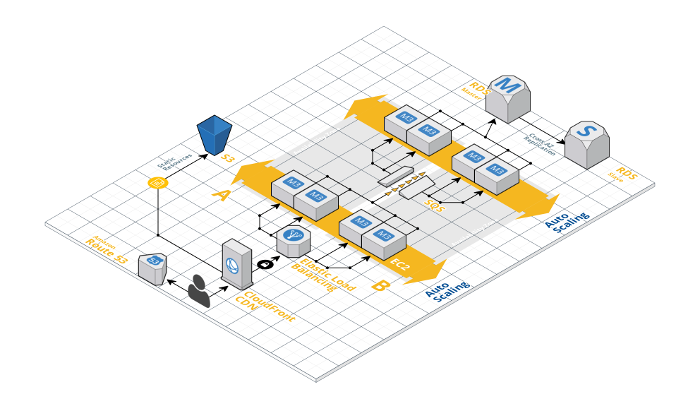
\includegraphics[width=0.8\textwidth]{resources/chapter-2-infrastructure-diagram.png}
        \caption{Contoh gambar}
        \label{fig:contoh_gambar}
    \end{figure}

    \subsubsection{Tabel}

    Tabel juga merupakan float. Tabel~\ref{table:contoh_tabel} adalah contoh tabel.

    \begin{table}[htbp]
        \small
        \centering
        \caption{Contoh Tabel}
        \label{table:contoh_tabel}
        \begin{tabular}{ll}
            \toprule
            \multicolumn{1}{l}{\textbf{Contoh Judul Kolom}} & \multicolumn{1}{l}{\textbf{Nilai}}\\
            \midrule
            Besaran 1 & 12 meter          \\
            Besaran 2 & $360^\circ$       \\
            Besaran 3 & 0,2 meter         \\
            Besaran 4 & $1^\circ$         \\
            Besaran 5 & 8000 sampel/detik \\
            \bottomrule
        \end{tabular}
    \end{table}

    \subsection{Persamaan Matematika}

    \blindtext Persamaan~\eqref{eq:contoh_equation} adalah contoh persamaan matematika,

    \begin{align}
        c^2 = a^2 + b^2\,.
    \label{eq:contoh_equation}
    \end{align}
    
    Contoh penggunaan notasi custom,
    
    \begin{align}
        \bayes{x}{y}\,.
    \label{eq:contoh_equation_custom}
    \end{align}

\section{Persyaratan Desain}

\section{Konsep Desain}
\blindtext

    \chapter{ANALISIS DAN PERANCANGAN}

\section{Analisis Masalah}
\blindtext

\section{Solusi Umum}
\blindtext

\section{Rancangan Solusi}
\blindtext
    \chapter{EVALUASI DAN PEMBAHASAN}

\section{Tujuan Pengujian}
\blindtext

\section{Skenario Pengujian}
\blindtext

\section{Hasil Pengujian}
\blindtext

\section{Pembahasan}
\blindtext
    \chapter{PENUTUP}

\section{Kesimpulan}
\blindtext

\section{Saran}
\blindtext
    %----------------------------------------------------------------%

    % Daftar pustaka
    %\begingroup
    %    \renewcommand{\baselinestretch}{1.0}
    %    \printbibliography[heading=bibintoc]
    %\endgroup
    
    \clearpage
    \bibliographystyle{IEEEtran}
    \bibliography{references}
    
    % Before:
    % ---
    % Index
    % \appendix
    % \addcontentsline{toc}{part}{Lampiran}
    % \part*{Lampiran}
    % ---

    % Format judul bab lampiran
    \titleformat{\chapter}[hang]
      {\large\bfseries}
      {\chaptertitlename\ \thechapter}{1em}
        {\large\bfseries}
    \titlespacing*{\chapter}{0pt}{-1.5\baselineskip}{\parskip}
    
    \clearpage
    \begin{center}
        \topskip0pt
        \vspace*{\fill}
        \large\textbf{LAMPIRAN}\normalsize
        \vspace*{\fill}
    \end{center}
    \clearpage
    
    \begin{appendices}
        \chapter{Instrumen Pengujian}
        \chapter{Rincian Kasus Uji}
    \end{appendices}

\end{document}
